\documentclass[a4paper,11pt]{article}
\usepackage{amssymb}
\usepackage{booktabs}
\usepackage{geometry}
\usepackage{color}
\usepackage{hyperref}
\usepackage{listings}
\usepackage{graphicx}
\usepackage{float}
\usepackage{caption}
\usepackage{subcaption}
\usepackage[T1]{fontenc}


\graphicspath{{img/}}

\setlength\parindent{0cm}

\geometry{
	includeheadfoot,
	margin=2.54cm
}

\title{
	2IL76 Algorithms for Geographic Data Set 4 \\
}
\author{
	Tim van Dalen (0744839)
	\and
	Bram Kohl (0746107)
	\and
	Bart van Wezel (0740608)
}
\date{\today}

\begin{document}
	\maketitle
	
\section*{Exercise 3}
For every region (partly or fully) within the necklace, we place a point on the necklace, as close as possible to the center of the (full) region. Then we combine the points of the regions of the same type by calculating a point between them, which is weighted by the area the region takes within the necklace. The final circle on the necklace is placed as close as possible to this point.

Example: there are 3 regions of type X which have a part in the necklace. \\
We first determine for each region: a point on the necklace, such that the distance to the center of the region is the lowest.
In the example this are the points A,B,E,F.  \\
Then for the types which have more than one region in the necklace, we determine the factor for each region. 
We do this by dividing the size of that region, by the total size of that type. 
So for the left yellow region, this is $\frac{4}{5}$ and for the right region $\frac{1}{5}$. 
Now we multiply the points we found on the necklace for each region by that factor and take the sum of those points. 
So for the left yellow region, we found the point $(1,0.5)$ on the circle and factor  $\frac{4}{5}$. 
This points thus becomes $(0.8,0.4)$. 
For the right yellow region, we found the point $(2,2)$ on the circle and factor  $\frac{1}{5}$. 
This points thus becomes $(0.4,0.4)$. When we take the sum of these points, we get point C: $(1.2,0.8)$.
From this point we will again determine  a point on the necklace, such that the distance to point C is the lowest, which is D in this example.  \\

Then we place the rings for that type on their point on the necklace. For the yellow region this is D, for the red region E, for the blue region F. \\
\begin{figure}[H]
	\centering
	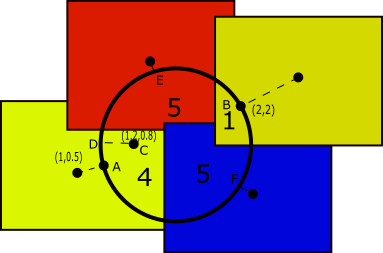
\includegraphics{figure1.png}
	\caption{Each pair of nodes is close enough, but no disk can be made}
	\label{fig:nodisk}
\end{figure}

When the rings of multiple regions intersect, we move the outer rings away till they can be placed without intersection.
So when three rings intersect, we move the two outer rings away. 
When two rings intersect we move away both rings till they can be placed without intersection. 
When there are more than three rings that intersect, we first move the outer two away and repeat this process till there are no intersections left. \\

We can continously move the circle, while still being spatially informative. 
When new regions join the necklace or old regions leave the necklace, they only take into account a small part of the total size of that type. 
This is because when a new region enters the necklace at first only a small part of that region is in the necklace and thus the factor of that region is still small. 
If we move the circle further into that region the factor increases and the label for that type changes its location slowly to that new region if that region is of significant size. 
When a old region leaves the necklace it already became smaller and smaller and thus the factor of that region got lower. 
This means the label of the type of that region already changed it's location to other regions of that type. 

\end{document}


